\chapter{Implementazione in matlab}
In quest'ultimo capitolo si mostrerà un'implementazione pratica degli algoritmi descritti.\\[0.5cm]
Fissiamo le notazioni: consideriamo il problema
$$
\begin{cases}
 y'(t)=f(t,y(t),y(t-\tau(t,y(t))))		\hspace{1cm}	t_0 \le t \le t_f	\\
 y(t)=\phi(t)					\hspace{5.1cm}	t \le t_0
\end{cases}
$$
per comodità di notazione poniamo
$$
s=t-\tau(t,y(t))
$$
quindi il problema viene riscritto come
$$
\begin{cases}
 y'(t)=f(t,y(t),y(s))			\hspace{1cm}	t_0 \le t \le t_f	\\
 y(t)=\phi(t)				\hspace{3.4cm}	t \le t_0
\end{cases}
$$
Sia $\Delta= \left \{ t_0, t_1, \dots, t_N=t_f \right \}$, allora seguendo l'algoritmo dei passi bisogna risolvere gli IVP

\begin{equation}
 \begin{cases}
 w_{n+1}'(t)	=	f(t,w_{n+1}(t),x(s)		\hspace{1cm}	t_n \le t \le t_{n+1}		\\
 w_{n+1}(t_n) 	=	 y_n
\end{cases}
\end{equation}
dove
$$
x(s)=
\begin{cases}
\begin{array}{c lc}
 \phi(s)		&	\mbox{se}	\hspace{1.2cm}		s \le t_0			\\	
 w_i(s)			&	\mbox{se}	\hspace{0.5cm}		t_i \le s \le t_{i+1}		\\
\end{array}
\end{cases}
$$
Pertanto è necessario risolvere $n$ IVP e la soluzione numerica che accettiamo è l'incollamento delle funzioni $\eta_i$ che 
sono gli interpolatori.\\[0.3cm]
Pertanto se $\eta_i$ è l'interpolatore della soluzione in $[t_i , t_{i+1}]$ allora possiamo scrivere 
la relazione

$$
\begin{cases}
\eta_0(t)=\phi(t)						\\
\eta_{i+1}'(t)=f(t,\eta_{i+1}(t),\eta_j(s))			\\
\eta_{i+1}(t_i)=\eta_i(t_i)
\end{cases}
$$
dove $j$ è tale che $s \in [t_j , t_{j+1}]$. Pertanto iterativamente vanno calcolate tutte le funzioni $\eta_i$.\\

\section{Codice}

\begin{lstlisting}[breaklines,caption={Implementazione del metodo dei passi per la risoluzione delle DDE}]
function [ mesh y ] = DDEsolver(  supmesh , history, tau, f, tol )

% input
% supmesh : suddivisione iniziale sulla quale avviare il metodo dei passi  
% history : storia della DDE
% tau : funzione ritardo
% f : definisce il problema
% tol : il numero di punti che deve avere la suddivisione (equispaziata) dei singoli IVP

% output
% mesh : suddivisione finale
% y : valutazioni della soluzione nella suddivisione mesh

% inizializzazione
y(1:length(supmesh),1:tol)=0;
mesh(1:length(supmesh),1:tol)=0;

% risoluzione del primo problema (caso base)

% storia con il ritardo
    function x = pasthistory(t,y)
        s=t-tau(t,y);
        x=history(s);
    end

% funzione ausiliaria che definisce il problema per past history

    function x = auxpasthistory(t,y)
        x=f(t,y,pasthistory(t,y));
    end

% calcolo della prima griglia di integrazione
mesh(1,:)=linspace(supmesh(1),supmesh(2),tol);

% calcolo della soluzione (discreta)
y(1,:)=ODEsolver(mesh(1,:),@auxpasthistory,history(supmesh(1)));

% funzione che interpola

    function x=interp(t)
        
        % ricerca dell'intervallo di appartenenza di t


        if (t<=supmesh(1))
            x=history(t);
        else
                        
            j=1;
            while(supmesh(j)<t)
                j=j+1;
            end
            j=j-1;
           
	  % interpolazione della soluzione
          x=interpolator(mesh(j,:),@pastinterp,t,y(j,:));
 
        end
    end

% funzione che interpola ritardata

    function x = pastinterp(t,y)
        
        % calcolo dell'argomento deviato
        s=t-tau(t,y);
        
        x=interp(s);
        
    end

% funzione che definisce il problema

    function x=aux(t,y)
        
        % calcolo dell'argomento deviato
        s=t-tau(t,y);
        
        x=f(t,interp(t),interp(s));
        
    end

for i=2:1:length(supmesh)-1
    
    % calcolo della griglia di integrazione
    mesh(i,:)=linspace(supmesh(i),supmesh(i+1),tol);
    % calcolo della soluzione discreta
    y(i,:)=ODEsolver(mesh(i,:),@aux,y(i-1,tol));
    
end

% concatenazione dei vettori (soluzione)
z=[];
w=[];
for i=1:1:max(size(supmesh))-1
    
    z=[z, y(i,:)];
    w=[w, mesh(i,:)];
    
end

y=z;
mesh=w;

end
\end{lstlisting}
\newpage
Di seguito ci sono le funzioni ODEsolver che risolve un IVP con Runge-Kutta classico a 4 stadi e interpolator che è il suo rispettivo 
interpolatore

\begin{lstlisting}[breaklines,caption={Risolutore di IVP}]
function y = ODEsolver( mesh, f, y1 )

% punto iniziale
y(1)=y1;

for i=1:1:length(mesh)-1
    % tempo corrente
    t = mesh(i);
    
    % passo di discretizzazione corrente
    h=mesh(i+1)-mesh(i);
    
    % punti della submesh
    t1=t;
    t2=t+h/2;
    t3=t+h/2;
    t4=t+h;
    
    % calcolo degli Y
    Y1=y(i);
    Y2=y(i)+0.5*h*f(t1,Y1);
    Y3=y(i)+0.5*h*f(t2,Y2);
    Y4=y(i)+h*f(t3,Y3);
    
    % calcolo del punto y(i+1)
    y(i+1)=y(i)+h*(1/6*f(t1,Y1)+1/3*f(t2,Y2)+1/3*f(t3,Y3)+1/6*f(t4,Y4));
    
end

end
\end{lstlisting}

\newpage

\begin{lstlisting}[breaklines,caption={Interpolatore del metodo}]
function eta = interpolator( mesh , f , t, y )

theta=2;
i=1;

h=mesh(2)-mesh(1);

while( (theta<0 || theta >1) && i < max(size(mesh)) )
    % tempo corrente in cui valutare l'interpolatore
    tn=mesh(i);
    
    % passo di discretizzazione corrente
    h=mesh(i+1)-mesh(i);
    
    % valore di theta (deve esser compreso tra 0 ed 1)
    theta=(t-tn)/h;
    
    i=i+1;
end

i=i-1;

% punti della submesh
t1=t;
t2=t+h/2;
t3=t+h/2;
t4=t+h;
    
% calcolo degli Y
Y1=y(i);
Y2=y(i)+0.5*h*f(t1,Y1);
Y3=y(i)+0.5*h*f(t2,Y2);
Y4=y(i)+h*f(t3,Y3);
    
eta=y(i)+h*((-1/2*theta+2/3)*theta * f(t1,Y1)+ 1/3*theta*f(t2,Y2)+ 1/3*theta*f(t3,Y3)+(1/2*theta-1/3)*theta*f(t4,Y4));


end
\end{lstlisting}
\vspace{1cm}
Si osservi che nel codice non ci sono tutti i controlli, si suppone ad esempio che la suddivisione $\Delta$ rispetti 
$t_{n+1}-t_n < \min \tau$ e al tempo stesso contenga tutte le discontinuità di grado al più 4, quindi questo codice è di certo migliorabile, daltronde 
per una questione di leggibilità si preferisce in questo contesto lasciarlo tale dato che lo si userà solo per fare esempi sugli errori.



\section{Esperimenti numerici}
Nel capitolo precedente si è dimostrato che utilizzando un metodo consistente e convergente per risolvere una DDE, sotto l'ipotesi 
che le discontinuità della soluzione siano incluse nella griglia $\Delta$, la soluzione numerica è una buona stima della soluzione, per 
l'esattezza l'errore è dello stesso ordine della convergenza del metodo usato.
\vspace{0.5cm}\\
Se le discontinuità non sono incluse in $\Delta$ a priori la soluzione numerica potrebbe non essere 
una buona stima della soluzione o per lo meno non si hanno risultati sull'ordine di convergenza del metodo.
Di seguito sono proposti degli esperimenti numerici realizzati con matlab usando il codice della sezione precedente,
 questi hanno il fine di mostrare quanto sia importante includere 
le discontinuità nella griglia.

\begin{exm}
Si consideri la DDE seguente (esempio 2.1)
$$
\begin{cases}
 y'(t)=-y(t-1)		 	\hspace{1cm} 		t \in [0,3]	\\
%  y(t)=1				\hspace{2.4cm}		t \le 0
\end{cases}
$$ 
Non è difficile scrivere la soluzione di questo problema, ad esempio usando il metodo dei passi, in $[0 , 3]$ la soluzione è
$$
y(t)=
\begin{array}{lc lc}
\begin{cases}
\displaystyle
1-t												&	\hspace{0.7cm}	0 \le t \le 1	\\
\displaystyle
\frac{t^2}{2}-2t+\frac{3}{2}									&	\hspace{0.7cm}	1 \le t \le 2	\\
\displaystyle
-\frac{t^3}{6}+\frac{3}{2}t^2-4t+\frac{17}{6}							&	\hspace{0.7cm}	2 \le t \le 3	\\
\end{cases}
\end{array}
$$
Si voglia ora determinare la soluzione numerica utilizzando l'approccio standard, come metodo numerico si può utlizzare  
Runge-Kutta classico con relativa estensione continua, questo è convergente di ordine $4$ e l'estensione continua è convergente di ordine $2$.

\begin{center}
\renewcommand\arraystretch{1,5}
\begin{tabular}{c|cccc}
 $0$			&	$0$			&	$0$			&		$0$		&	$0$		\\
 $\frac{1}{2}$		&	$\frac{1}{2}$		&	$0$			&		$0$		&	$0$		\\
 $\frac{1}{2}$		&	$0$			&	$\frac{1}{2}$		&		$0$		&	$0$		\\
 $1$			&	$0$			&	$0$			&		$1$		&	$0$		\\
\hline
			&	$\frac{1}{6}$		&	$\frac{1}{3}$		&	$\frac{1}{3}$		&	$\frac{1}{6}$	\\
\end{tabular}
\renewcommand\arraystretch{1}
\hspace{2cm}
$
\renewcommand\arraystretch{1,5}
\begin{array}{lc}
 b_1(\theta) = \left( -\frac{1}{2} \theta + \frac{2}{3} \right) \theta						\\
 b_2(\theta) = \frac{1}{3} \theta										\\
 b_3(\theta) = \frac{1}{3} \theta										\\
 b_4(\theta) = \left( \frac{1}{2} \theta - \frac{1}{3} \right) \theta
\end{array}
\renewcommand\arraystretch{1}
$
\end{center}



Le discontinuità della soluzione sono localizzate negli interi, quindi ai fini della convergenza della soluzione numerica alla 
soluzione, bisogna che $ \left \{ 0,1,2,3 \right \} \in \Delta$.\vspace{0.5cm}\\
Essendo nota la soluzione del problema è possibile calcolare l'errore assoluto, dunque utilizzando il metodo appena descritto, scegliendo 
$\Delta= \left \{ 0 , 1 , 2 , 3 \right \}$ e come $\Delta'= \left \{ 0 , 0.5 , 1.3 , 2.2 , 3 \right \}$, posto $h=(t_{i+1}-t_i)/N$ (ovvero 
nella risoluzione dell'IVP consideriamo la suddivisione equispaziata) otteniamo in scala logaritmica

% da un warning
\begin{center}
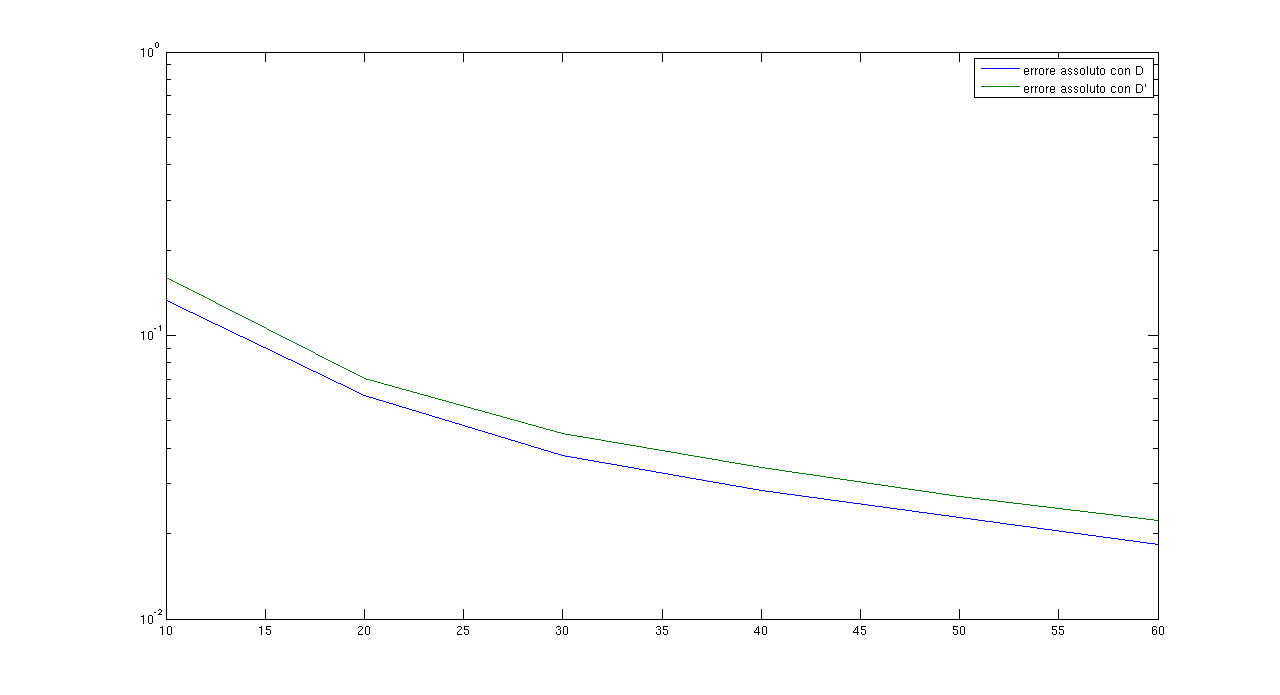
\includegraphics[width=15cm]{immagini/immagine10.png}
\end{center}
% fine warning

Quindi è evidente che nel caso in si sceglie $\Delta$ il metodo è convergente di ordine 2, mentre se si sceglie $\Delta$ la convergenza è più lenta
\begin{center}
\begin{tabular}{|c|c|c|}
\hline
 N	&	errore con $\Delta$	&	errore con $\Delta'$	\\
\hline
10	&	0.1329			&	0.1600			\\
\hline
20	&	0.0613			&	0.0707			\\
\hline
30	&	0.0377			&	0.0450			\\
\hline
40	&	0.0283			&	0.0344			\\
\hline
50	&	0.0227			&	0.0270			\\
\hline
60	&	0.0184			&	0.0223			\\
\hline
\end{tabular}
\end{center}

Daltronde questo è un esempio fortunato come in generale il caso delle DDE con ritardo costante, infatti con l'incremento di $N$ l'errore assoluto 
con $\Delta$ e $\Delta'$ tende ad esser lostesso. L'esempio che segue mostra un comportamente decisamente peggiore.
\end{exm}
\vspace{1cm}
\begin{exm}[\cite{4}]

 Si consideri la seguente DDE
$$
\displaystyle
\begin{cases}
\displaystyle
 y'(t)=\frac{1}{2 \sqrt{t}} y \left( y(t)-\sqrt{2} +1  \right)		 	\hspace{1cm} 		t \in [1,3]	\\
 y(t)=1										\hspace{4.7cm}		t \le 1
\end{cases}
$$
La soluzione di questa DDE è la seguente
$$
y(t)=
\begin{cases}
\begin{array}{lc c}
\displaystyle
 \sqrt{t}										&	\hspace{1cm}		1 \le t \le 2	\\
\displaystyle
 \frac{t}{4}+\frac{1}{2}+\left( 1 - \frac{\sqrt{2}}{2} \right) \sqrt{t}			&	\hspace{1cm}		2 \le t \le 3
\end{array}
\end{cases}
$$
Si consideri il seguente metodo di Runge-Kutta con relativo interpolatore

\begin{center}
\renewcommand\arraystretch{1,5}
\begin{tabular}{c|cccc}
 $0$			&	$0$			&	$0$			&		$0$	\\
 $\frac{1}{3}$		&	$\frac{1}{3}$		&	$0$			&		$0$	\\
 $\frac{2}{3}$		&	$0$			&	$\frac{2}{3}$		&		$0$	\\
\hline
			&	$\frac{1}{4}$		&	$0$			&	$\frac{3}{4}$	\\
\end{tabular}
\renewcommand\arraystretch{1}
\hspace{2cm}
$
\renewcommand\arraystretch{1,5}
\begin{array}{lc}
 b_1(\theta) = -\frac{3}{4} \theta^2 + \theta									\\
 b_2(\theta) = 0												\\
 b_3(\theta) = \frac{3}{4} \theta^2
\end{array}
\renewcommand\arraystretch{1}
$
\end{center}
Questo metodo è convergente di ordine 3 e l'estensione continua è convergente di ordine 2.
\\[0.5cm]
La soluzione della DDE ha una discontinuità in 2, quindi ai fini della convergenza è necessario includerle 2 nella suddivisione, daltronde è possibile 
fare scelte particolarmente sbagliate, infatti se si vuol risolvere il problema in $[1, 3.11111]$ allora ogni suddivisione $\Delta$ equispaziata 
provoca la propagazione della discontinuità in ogni intervallo di integrazione. Si considerino dunque le due suddivisioni: 
$\Delta=\left \{1,1.5, 2, 2.5, 3.11111 \right \}$ e $\Delta' = \left \{ 1, 1.7037, 2.4074, 3.1111 \right \}$


% da un warning
\begin{center}
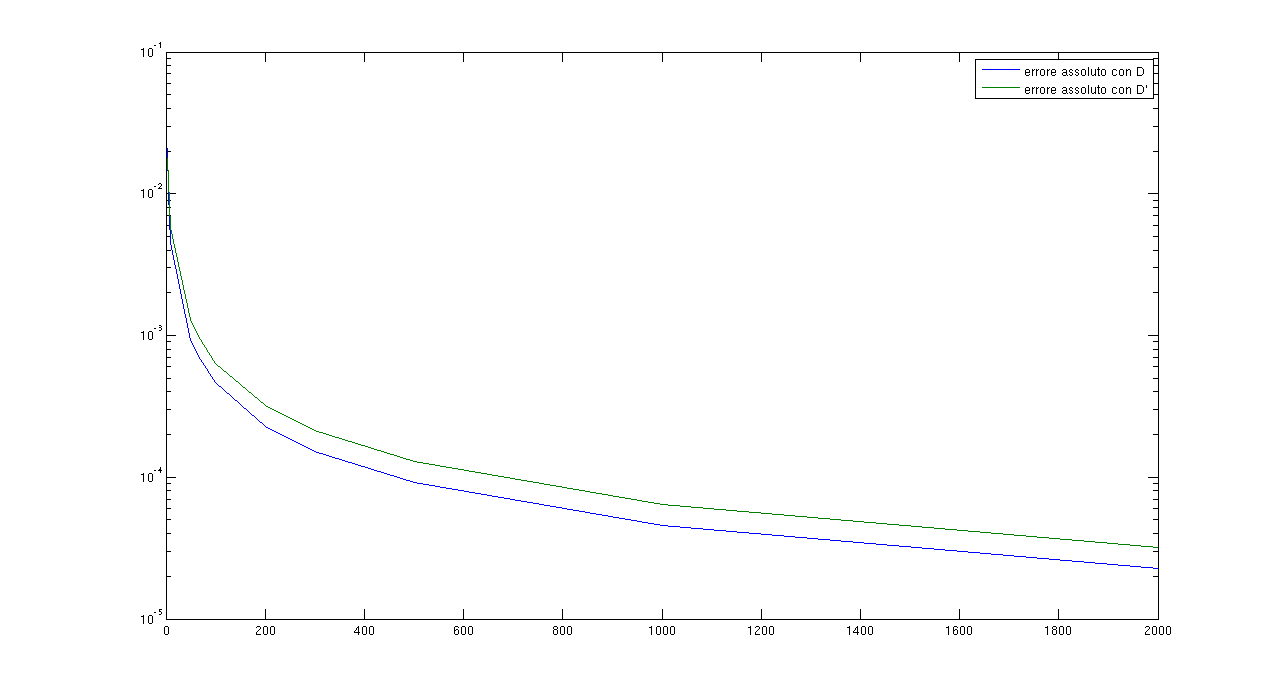
\includegraphics[width=15cm]{immagini/immagine11.png}
\end{center}
% fine warning

Si osserva che in accordo con il teorema 4.1 la convergenza del metodo dei passi è di ordine 3 se si sceglie $\Delta$, mentre con $\Delta'$ è di 
ordine 2.


\begin{center}
\begin{tabular}{|c|c|c|}
\hline
 N	&	errore con $\Delta$	&	errore con $\Delta'$	\\
\hline
3	&	0.020991262384127			&	0.017744352867936			\\
\hline
5	&	0.010278532116582			&	0.012465780914469			\\
\hline
10	&	0.004512684162531			&	0.005750132670051			\\
\hline
50	&	0.000918383645406			&	0.001287267751515			\\
\hline
70	&	0.000677030564511			&	0.000940632930354			\\
\hline
100	&	0.000465559043085			&	0.000633592107134			\\
\hline
200	&	0.000229255749912			&	0.000318725862569			\\
\hline
300	&	0.000151769755634			&	0.000213068390289			\\
\hline
500	&	0.000091428520250			&	0.000128912477018			\\
\hline
\end{tabular}
\end{center}

Quindi anche con $N$ molto grande la scelta della suddivisione continua ad influire sull'ordine di convergenza.
\end{exm}
